\documentclass[12pt]{article}
\setlength{\oddsidemargin}{0in}
\setlength{\evensidemargin}{0in}
\setlength{\textwidth}{6.5in}
\setlength{\parindent}{0in}
\usepackage{graphicx}
\usepackage{multirow}
\usepackage{multicol}
\usepackage{listings}
\usepackage{color}

\definecolor{dkgreen}{rgb}{0,0.6,0}
\definecolor{gray}{rgb}{0.5,0.5,0.5}
\definecolor{mauve}{rgb}{0.58,0,0.82}

\lstset{frame=tb,
  language=MATLAB,
  aboveskip=3mm,
  belowskip=3mm,
  showstringspaces=false,
  columns=flexible,
  basicstyle={\small\ttfamily},
  numbers=none,
  numberstyle=\tiny\color{gray},
  keywordstyle=\color{blue},
  commentstyle=\color{dkgreen},
  stringstyle=\color{mauve},
  breaklines=true,
  breakatwhitespace=true,
  tabsize=3
}

\usepackage{amsmath,amssymb,amsrefs, array}

\usepackage[top=24mm, bottom=18mm, left=15mm, right=13mm]{geometry}
\usepackage{url}

\title{Project 2 Report}
\author{Lawrence Ouyang}

\begin{document}
\maketitle
\section{User Guide}
Included with this project are the following two MATLAB files:
\begin{itemize}
\item project2main.m
\item ConjugateGradientPDE\_2D.m
\end{itemize}
\underline{\textit{project2main.m}} is a script which solves exactly what the specs are asking for, that is:
\begin{enumerate}
\item Solves the equation $-u_{xx} - u_{yy} + e^{x+y}u = 1$ for $ N = {32,64,128,256,512}$.
\item Plots the five graphs, one for each $N$.
\item Examines the relationship between $N$ and the number of iterations required to obtain the solution.
\end{enumerate}
\underline{\textit{ConjugateGradientPDE\_2D.m}} is the function that solves the equation
\[
-u_{xx} - u_{yy} + q(x,y)u = r(x,y)
\]
It has the following input variables in respective order:
\begin{itemize}
\item q\_xy: Function $q(x,y)$ of the equation
\item r\_xy: Function $r(x,y)$ of the equation
\item N: Size of parition of domain
\item TOL: Threshold value for relative residual
\item Iteration: Maximum number of iterations until program terminates
\end{itemize}
And the following outputs in respective order:
\begin{itemize}
\item u: Solution matrix of size $(N-1) \times (N-1)$.
\item k: Number of iterations required to obtain u.
\end{itemize}
\newpage
\section{Solutions}
The plots of the graphs are shown below and on the next pages: \\
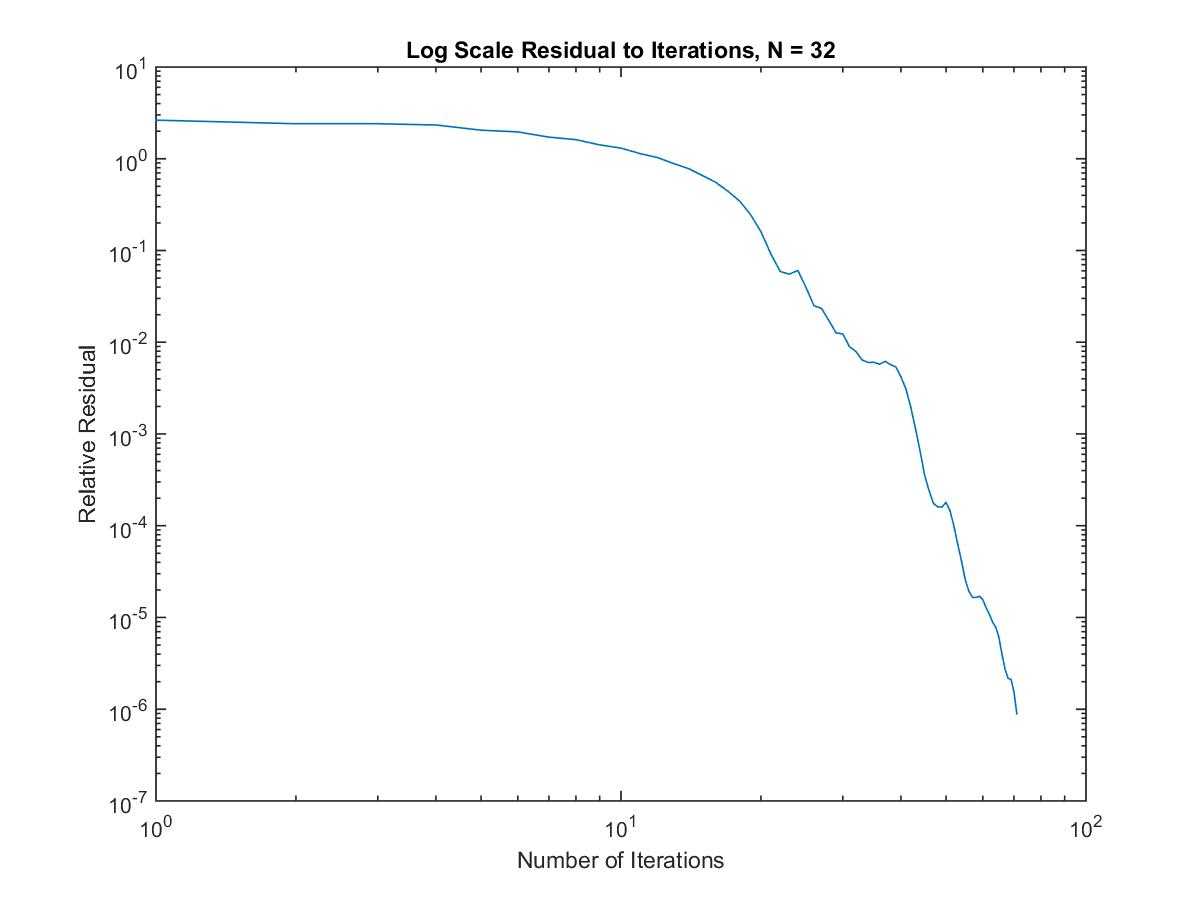
\includegraphics[scale = 0.35]{logplotN-32.jpg} \\
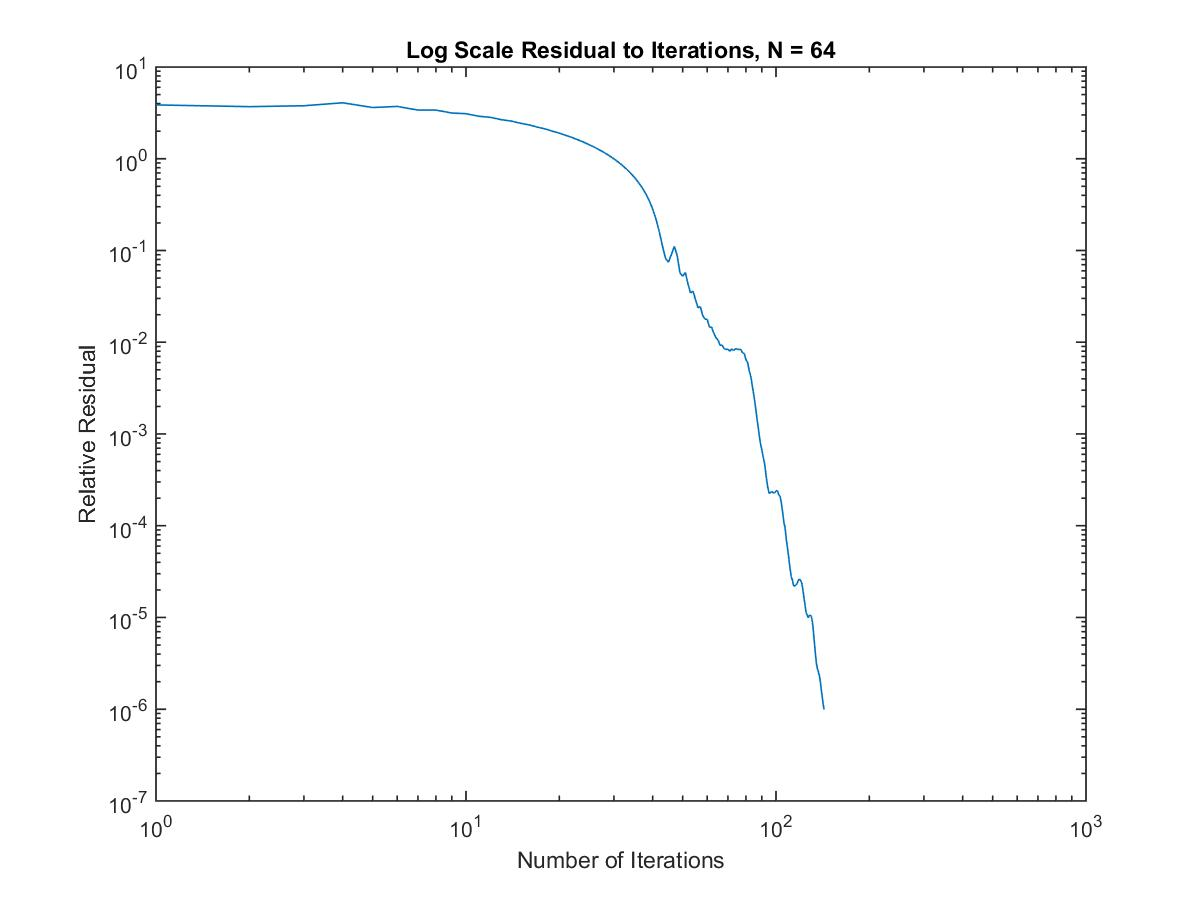
\includegraphics[scale = 0.35]{logplotN-64.jpg} \\
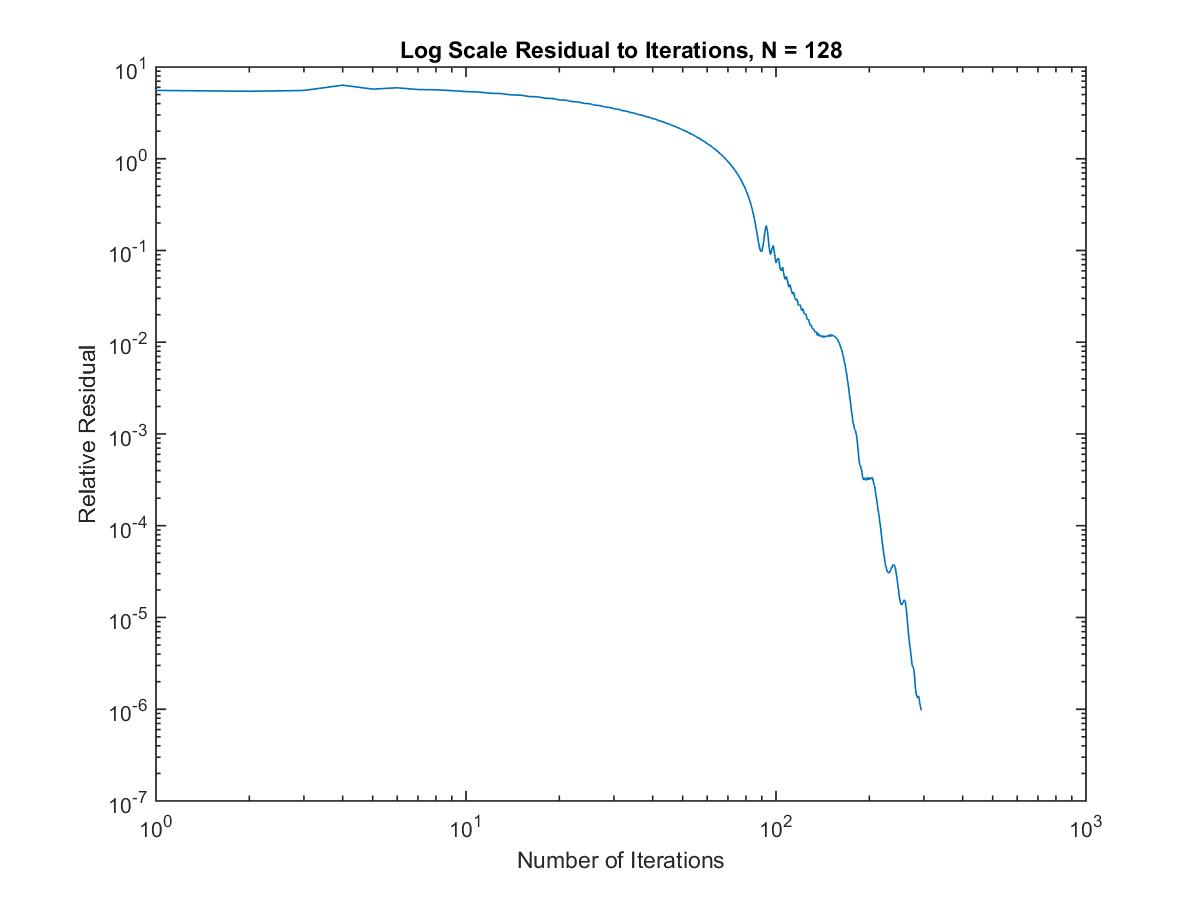
\includegraphics[scale = 0.35]{logplotN-128.jpg} \\
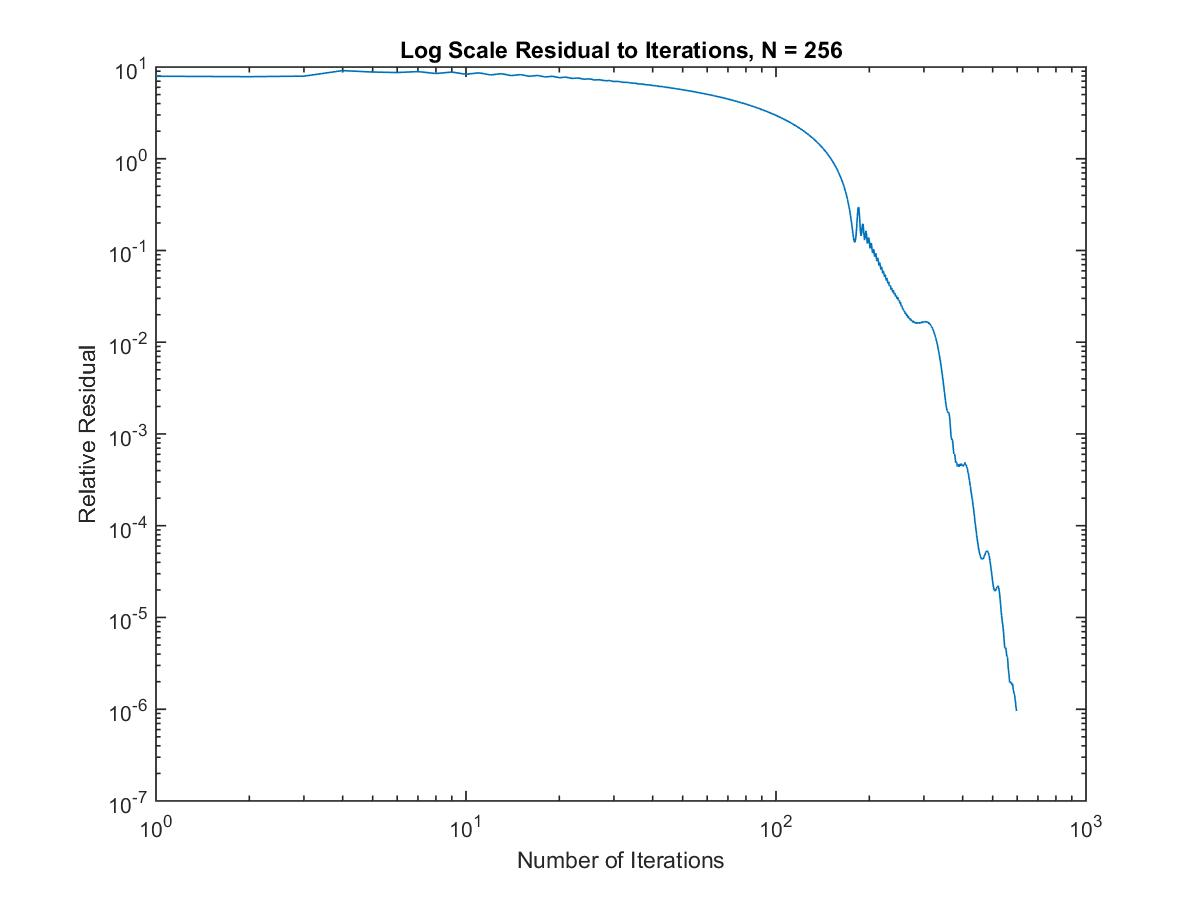
\includegraphics[scale = 0.35]{logplotN-256.jpg} \\
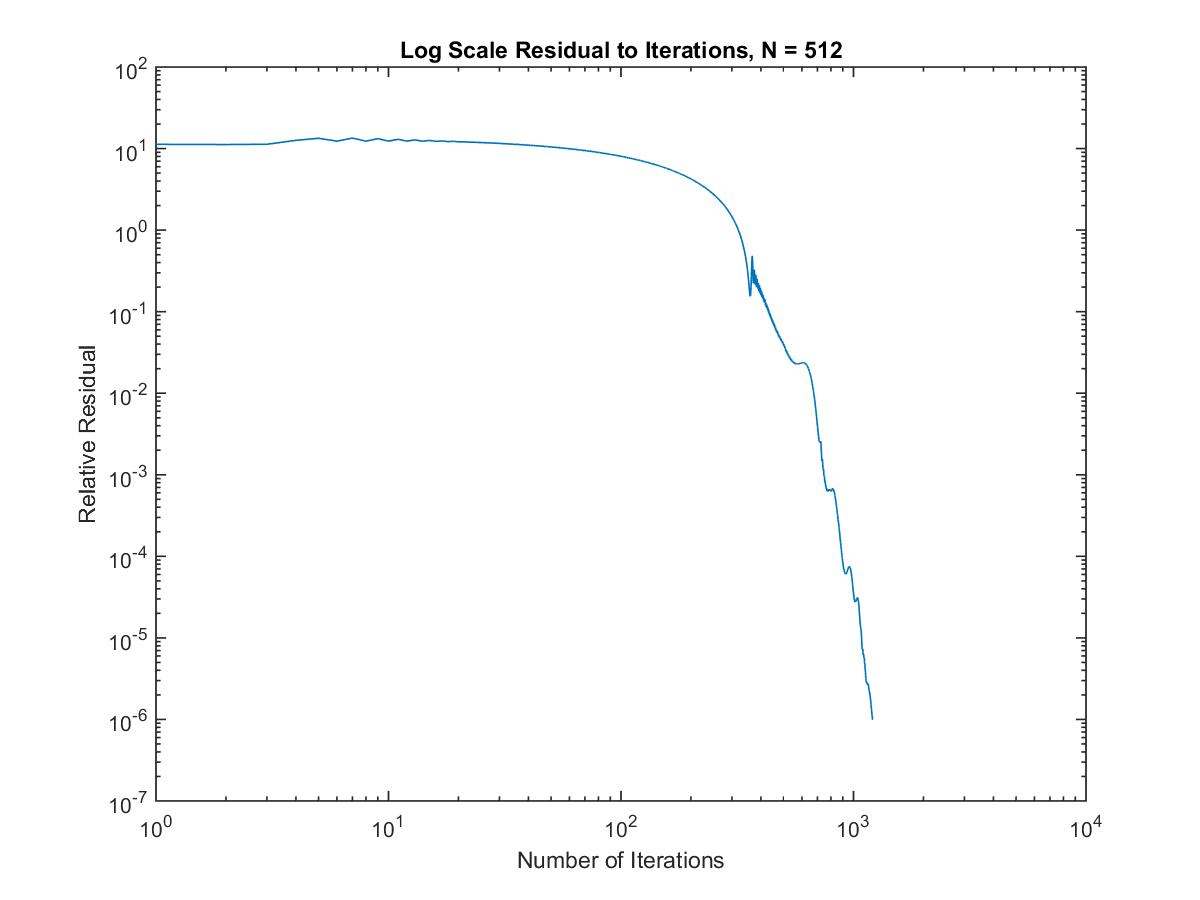
\includegraphics[scale = 0.35]{logplotN-512.jpg} \\
The table below shows how many iterations each N needed:\\
\begin{center}
\begin{tabular}{|c||c|c|c|c|c|}
\hline
$N$ & 32 & 64 & 128 & 256 & 512 \\
\hline
$k$ & 71 & 143 & 294 & 597 & 1208 \\
\hline
\end{tabular}
\end{center}
\newpage
\section{Discussion}
An obvious relationship can be seen just by examining the table in the solutions section. As $N$ increases, the number of iterations $k$ also increases, approximately at the same rate as N. Below is the Logarithmic Scaled graph of $k$ and $N$ and describes an increasing linear slope: \\
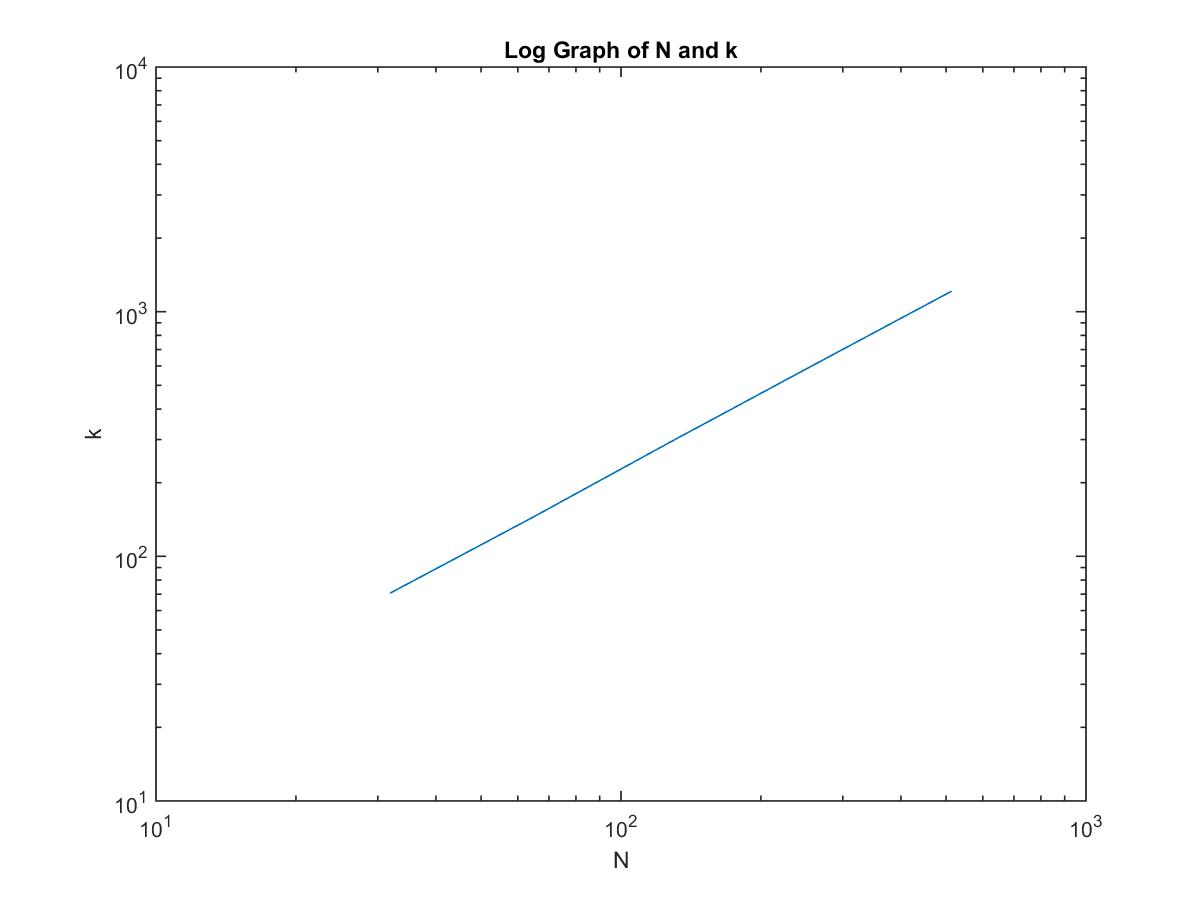
\includegraphics[scale = 0.45]{logplotN-k.jpg}
 
\end{document}